%!TEX root=../../main.tex


\subsection{The frameworks during setup and benchmark}
We would like to raise some issues we encountered first while installing and configuring and second while running the different frameworks.

\begin{enumerate}
	\item During setup of Gemini, we realized that the cloned repository contained several bugs, rendering the code as-is unable to perform any calculations. We had to fork and modify the source code. TODO(Was genau ging nicht, was haben wir geändert?)

	The repository with our changes can be found \href{https://github.com/jasc7636/GeminiGraph}{here}\footnote{\url{https://github.com/jasc7636/GeminiGraph}}.
	\item Furthermore, we would like to address the setup of Hadoop for Giraph. It requires multiple edits in \texttt{xml} files that aren't easily automized. This makes the setup rather time consuming, especially if reconfiguration is needed later on.
	\item Also in order for Giraph to run, several Java tasks have to be constantly running in the background. While we don't expect this to have a noticeable performance impact on other tasks, it is still not optimal.
	\item The Hadoop distributed file system (HDFS) ran us into disk space problems on multiple occasions. First, unless configured otherwise, the standard implementation replicates all data three times, distributed over all participating nodes. Second, deleting files on the HDFS does not immediately free up disk space because the files are moved to a \emph{recycling bin}-like location.

	\item 
\end{enumerate}


On a plus side, setup of frameworks like Polymer or Ligra was straight forward and did not require any special treatment. 





\subsection{Pure Performance-Ergebnisse}



\subsection{Ergebnisse Calc time}
\begin{figure}
	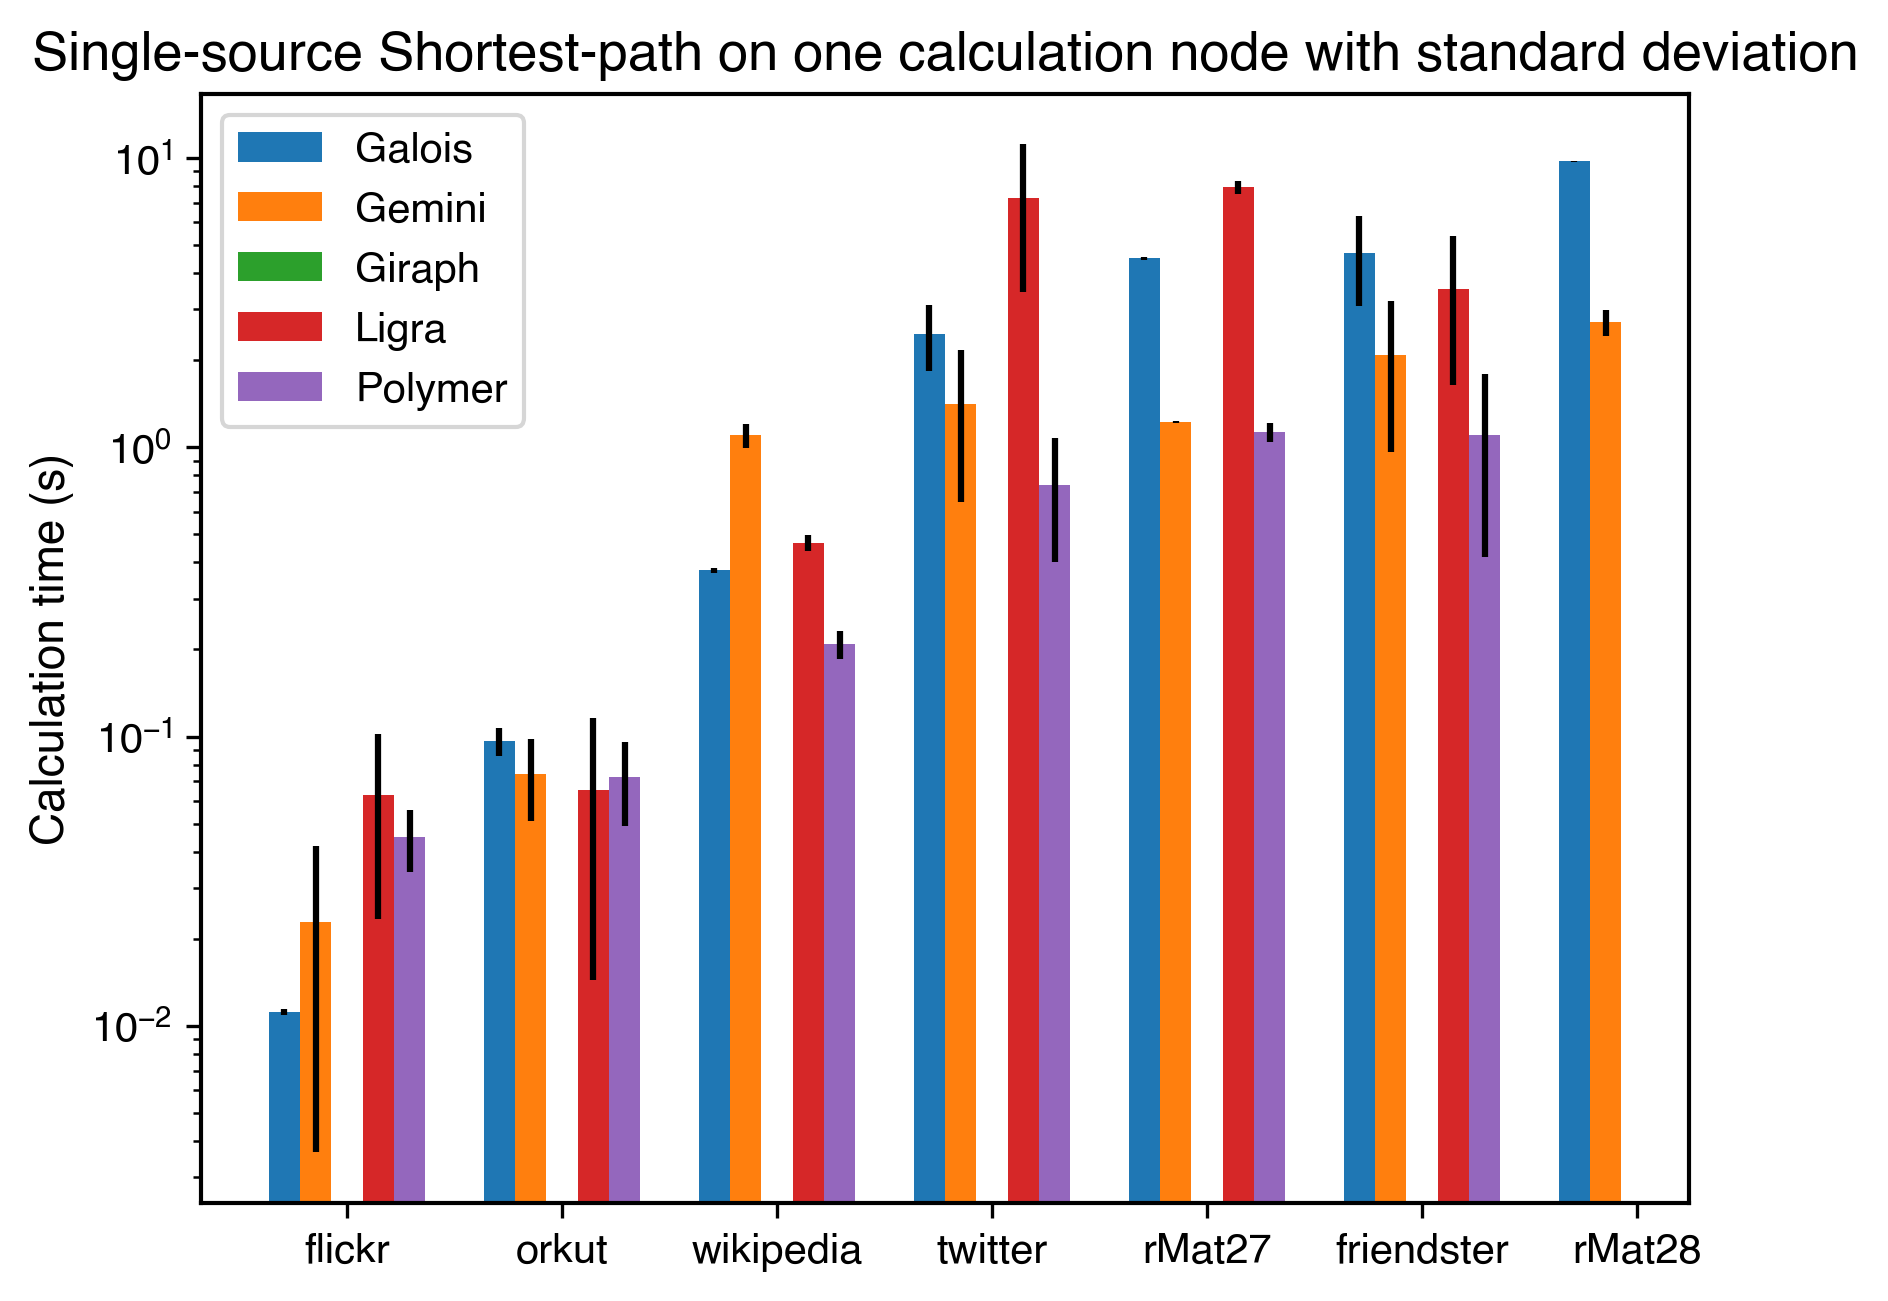
\includegraphics[width=\columnwidth]{../../plots/singleNodeSSSP_calcTime.png}
	\caption{Calculation times for SSSP on a single node}
	\label{fig:singleNodeSSSP_calc}
\end{figure}

\begin{figure}
	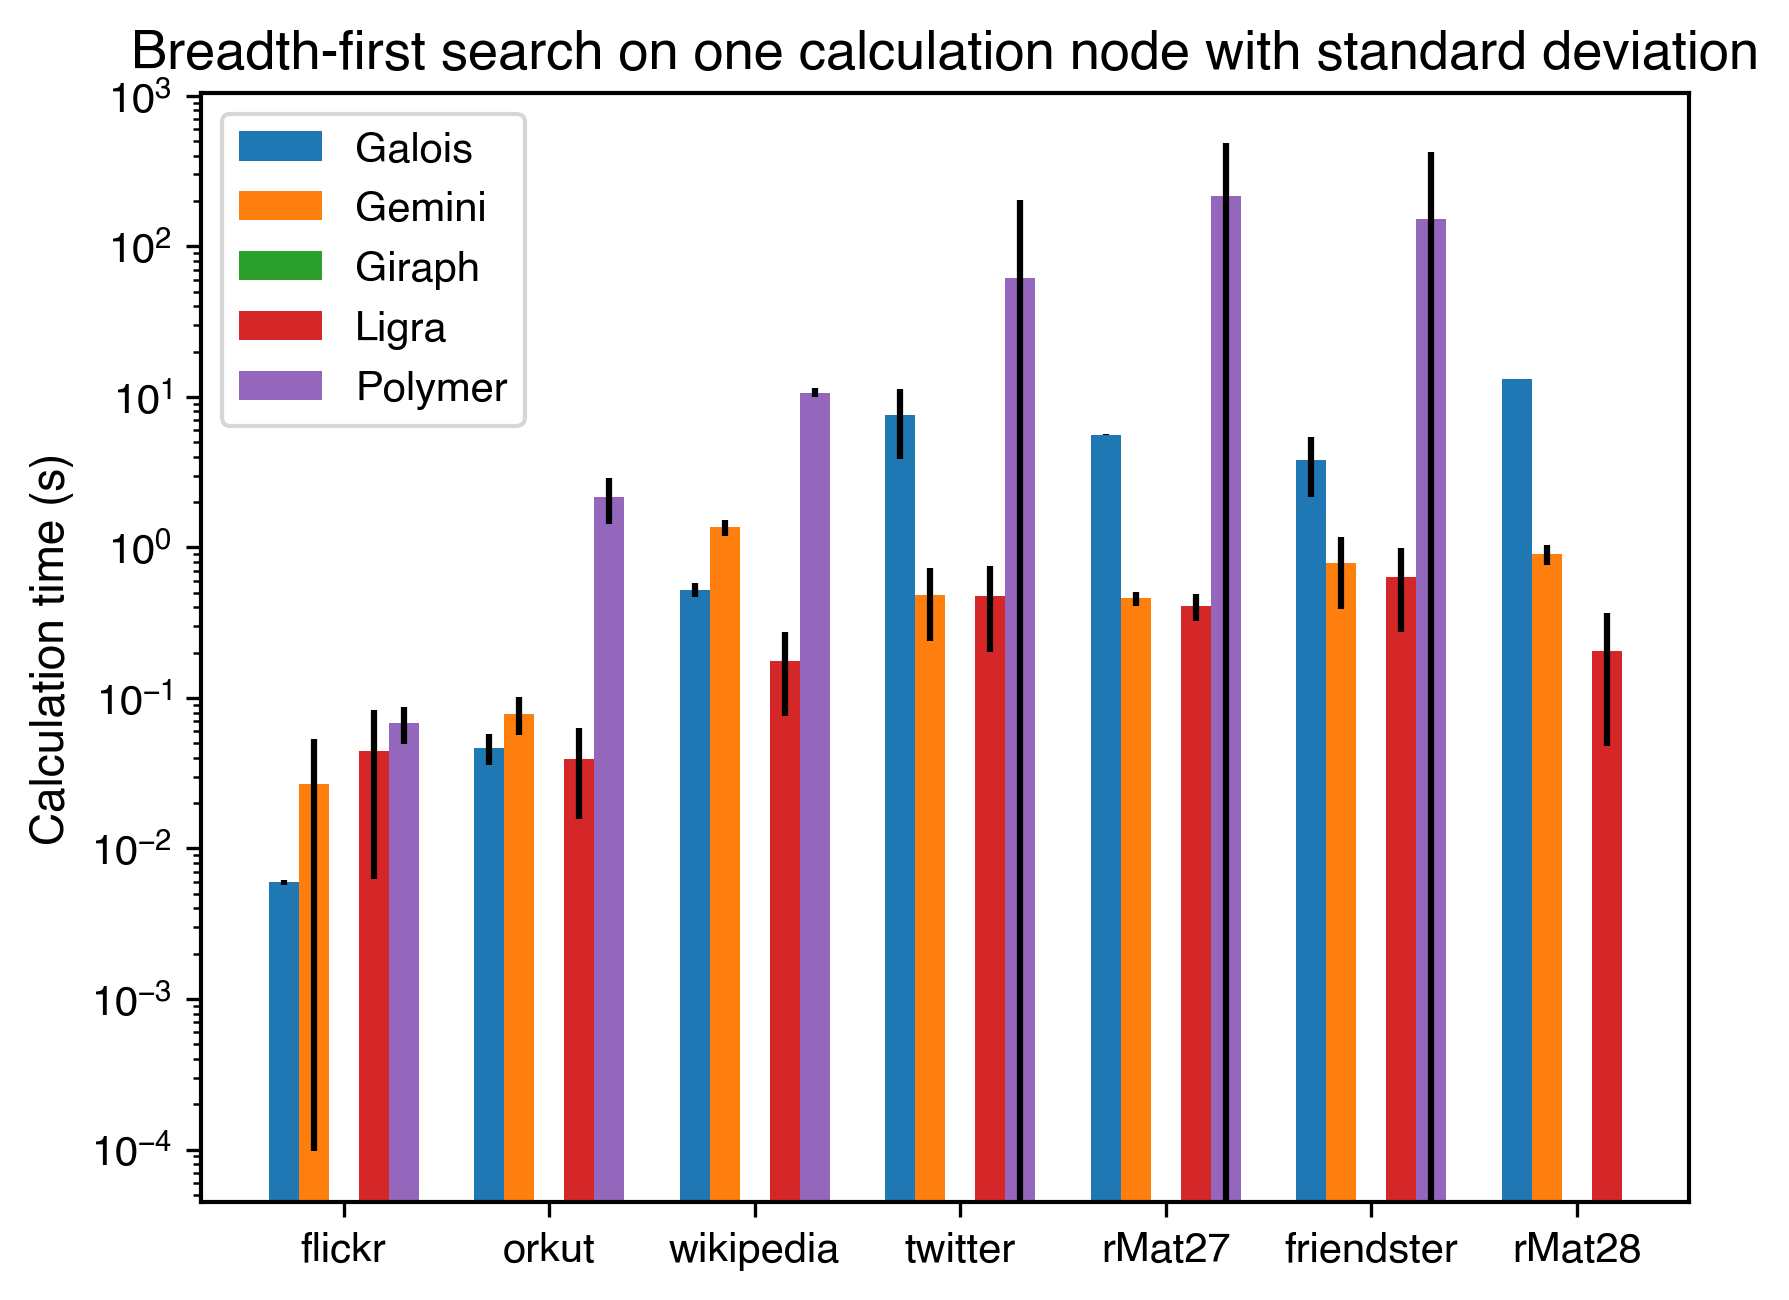
\includegraphics[width=\columnwidth]{../../plots/singleNodeBFS_calcTime.png}
	\caption{Calculation times for BFS on a single node}
	\label{fig:singleNodeBFS_calc}
\end{figure}

\begin{figure}
	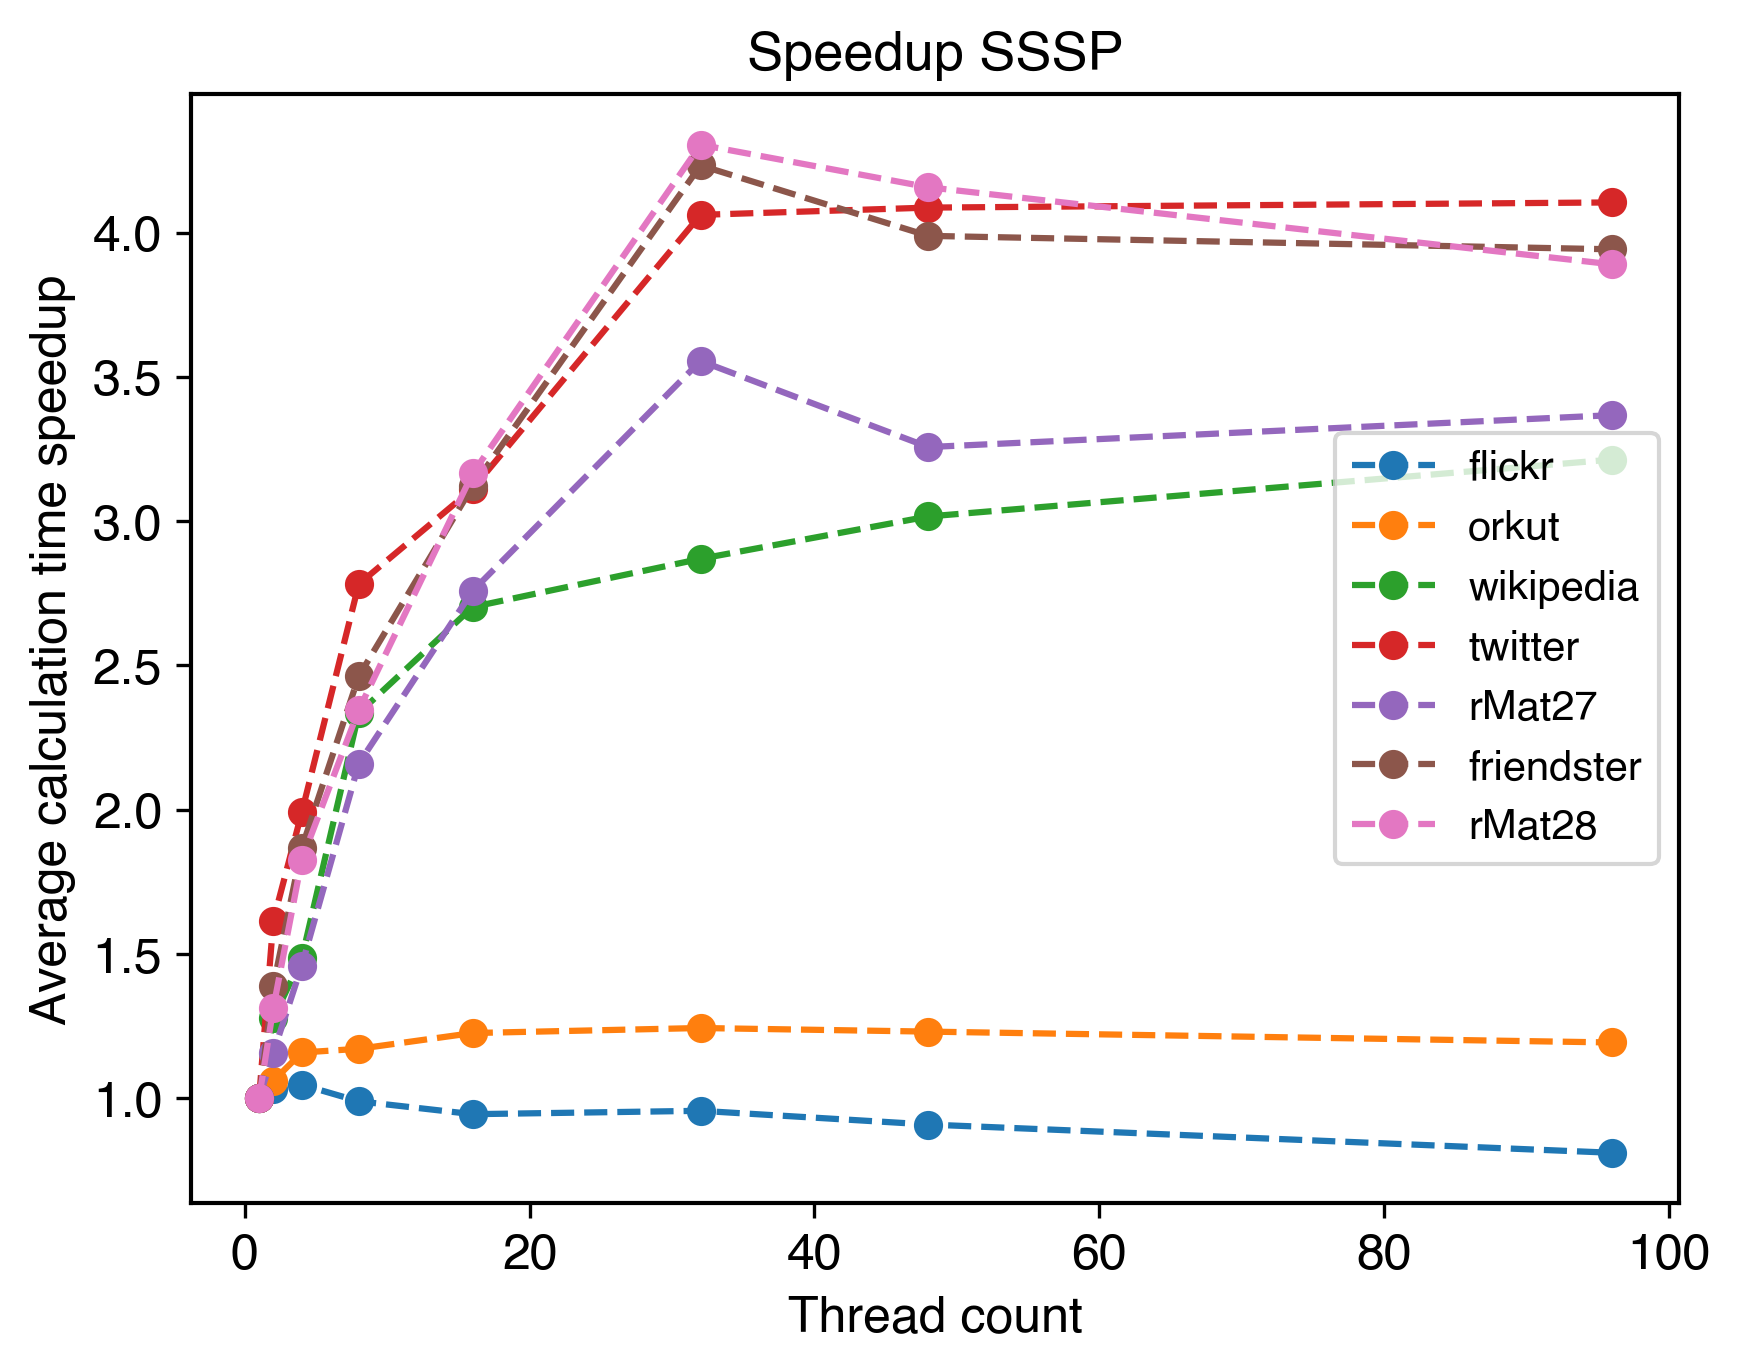
\includegraphics[width=\columnwidth]{../../plots/singleNodeSSSPGaloisThreads.png}
	\caption{Calculation times of Galois' SSSP over the thread count}
	\label{fig:singleNodeSSSPGaloisThreads}
\end{figure}





\subsection{Ergebnisse exec time}
\begin{figure}
	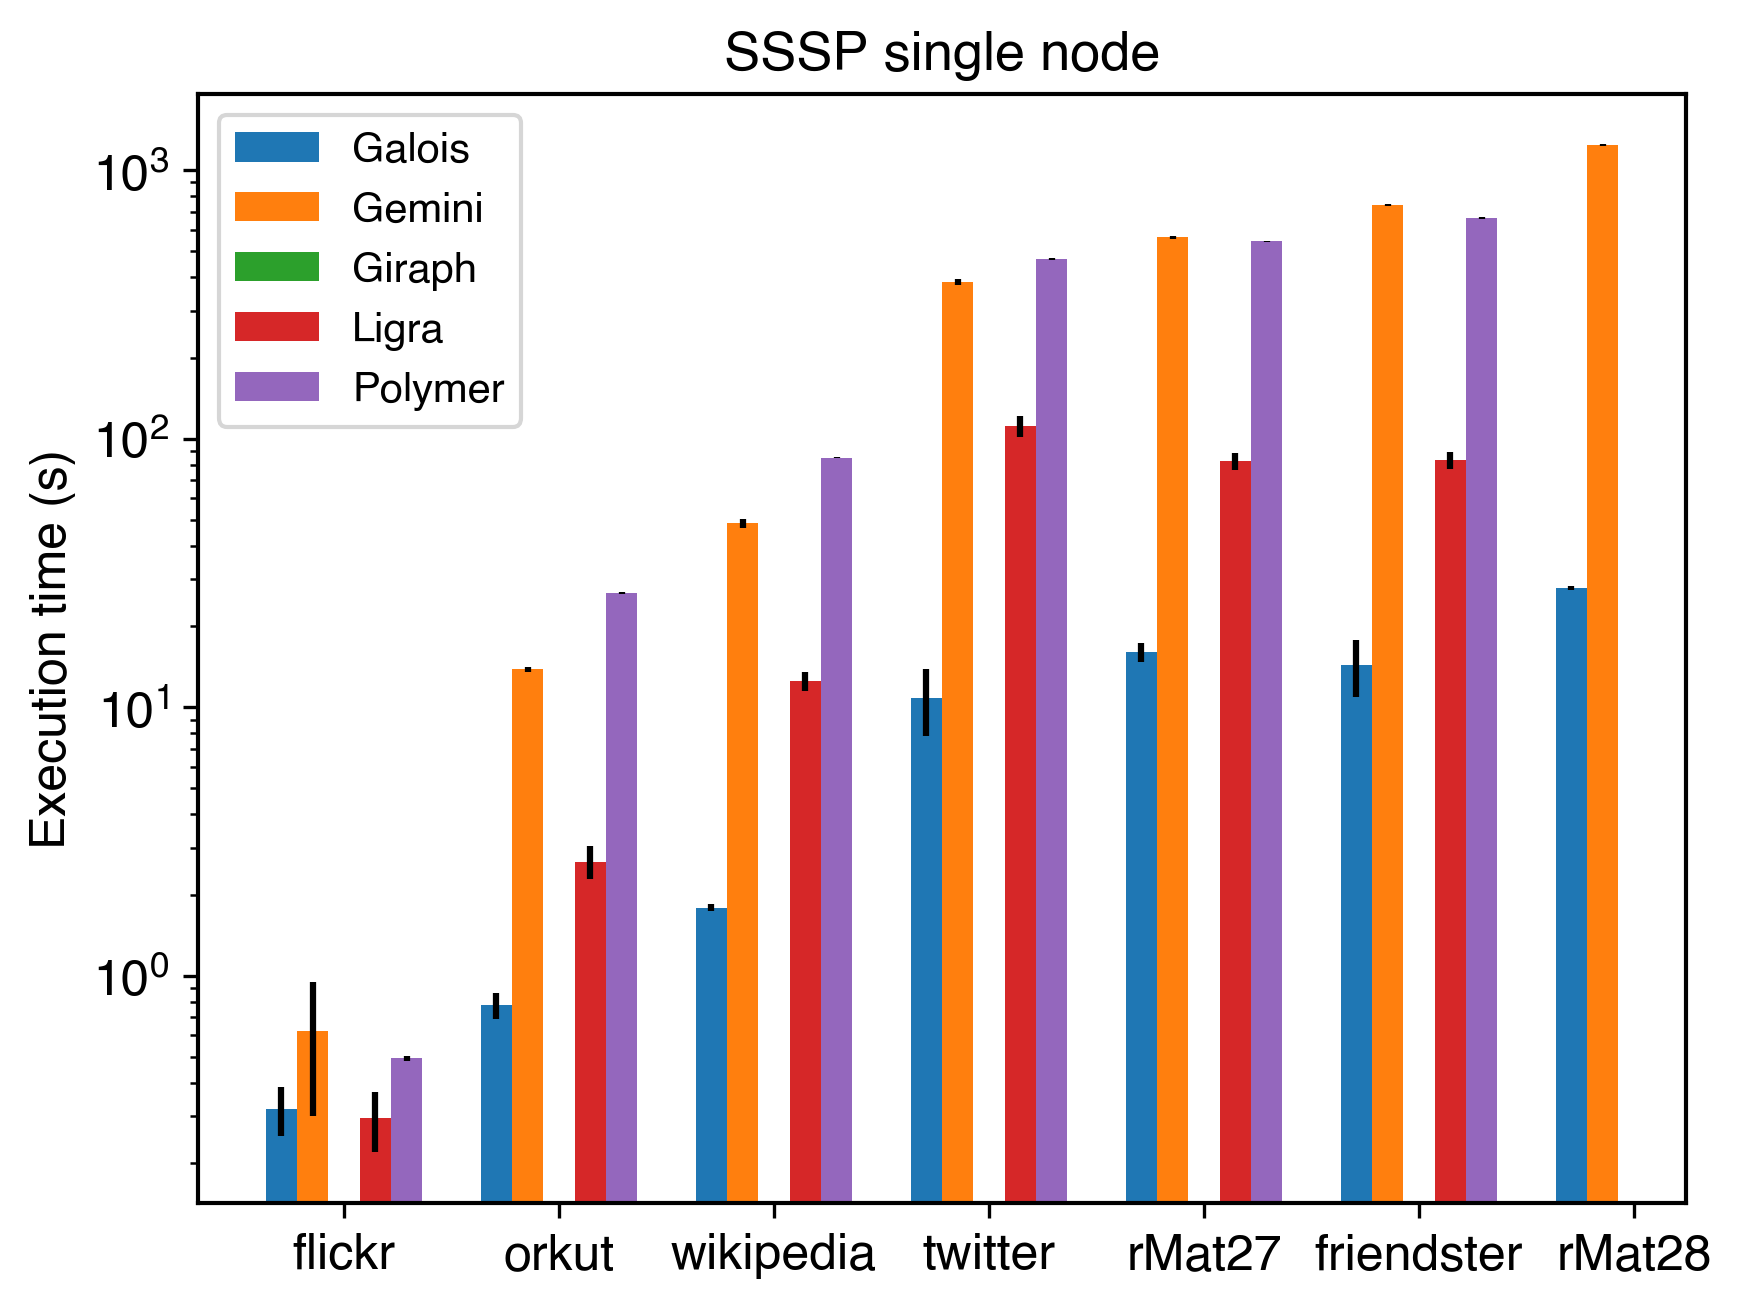
\includegraphics[width=\columnwidth]{../../plots/singleNodeSSSP_execTime.png}
	\caption{Execution times for SSSP on a single node}
	\label{fig:singleNodeSSSP_exec}
\end{figure}

\begin{figure}
	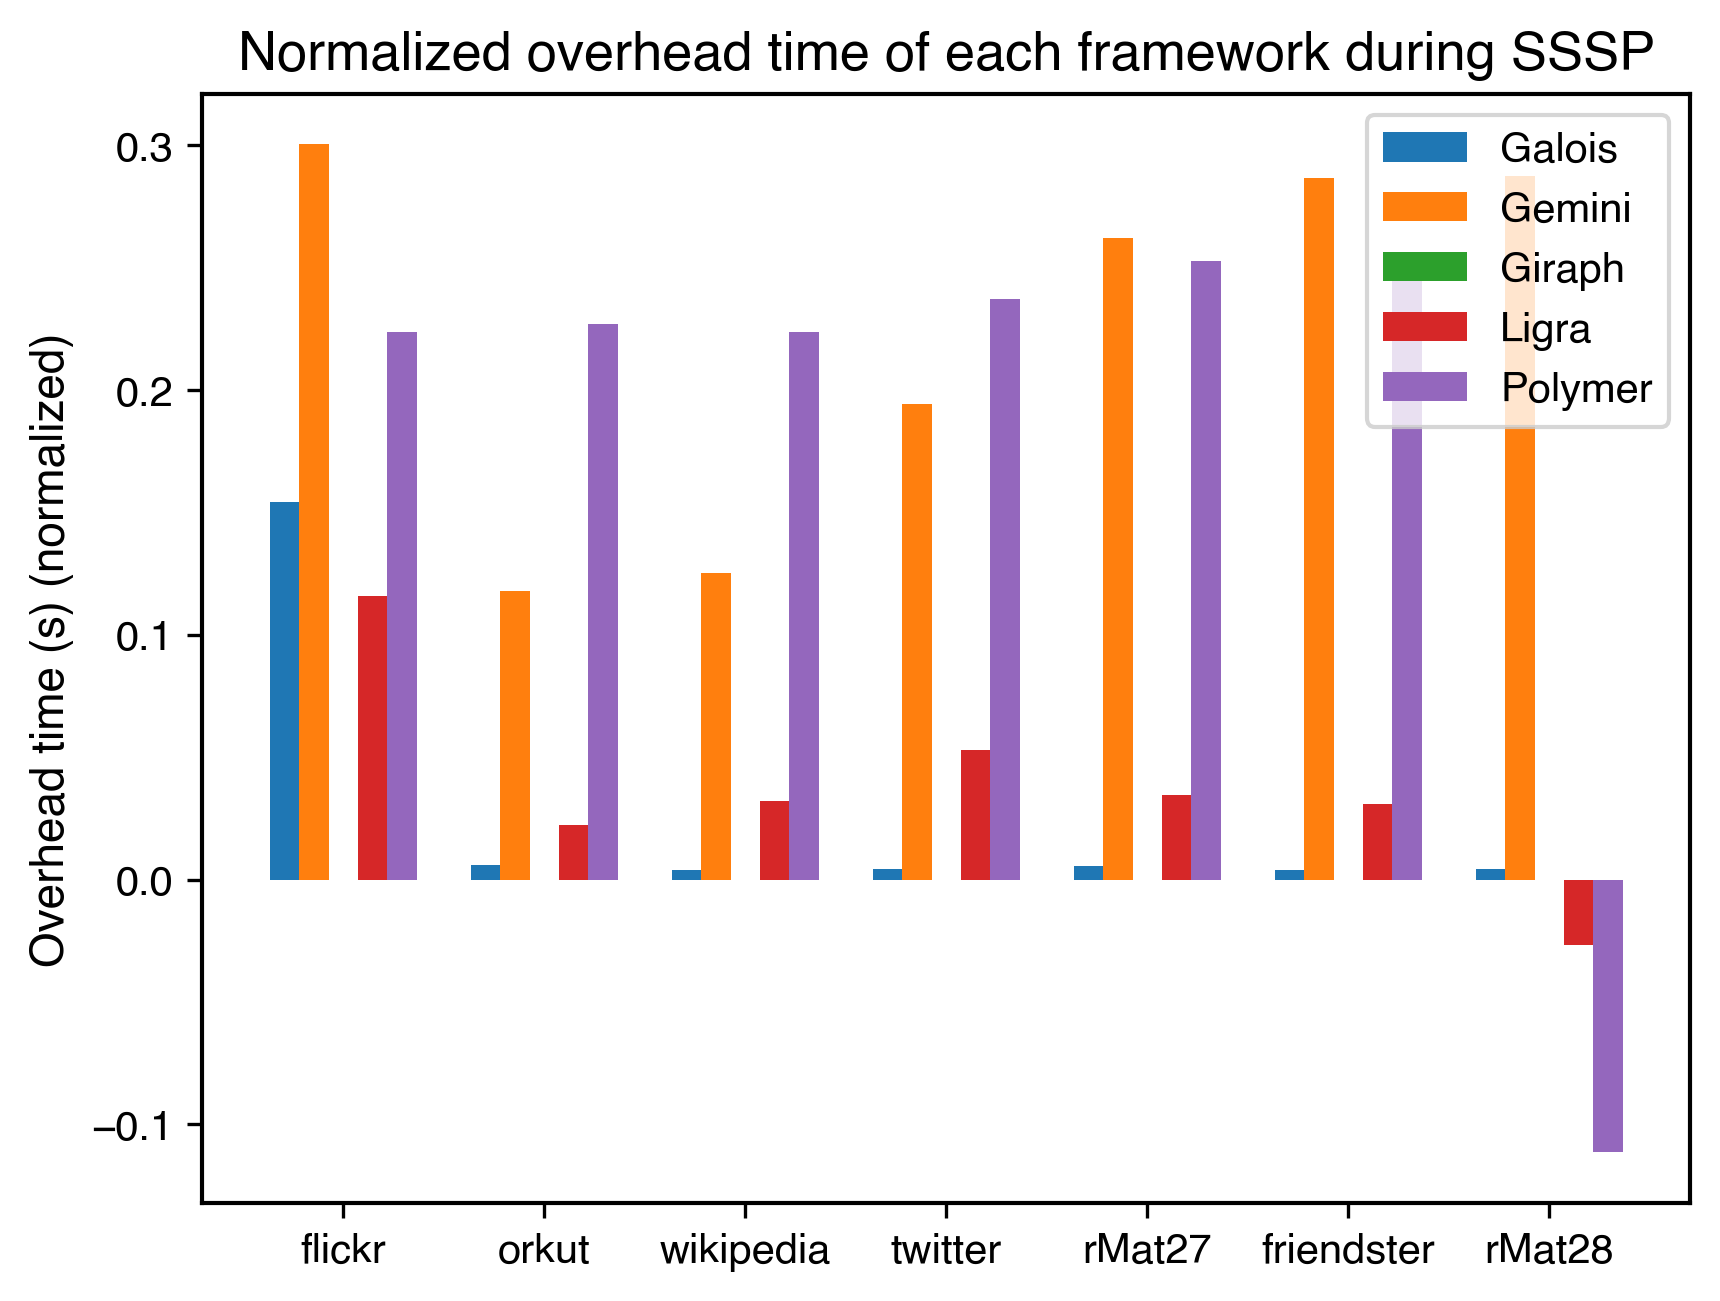
\includegraphics[width=\columnwidth]{../../plots/singleNodeSSSP_overheadTimeNormalized.png}
	\caption{Normalized Overhead SSSP single node}
	\label{fig:singleNodeSSSP_overheadNormalized}
\end{figure}

\begin{figure}
	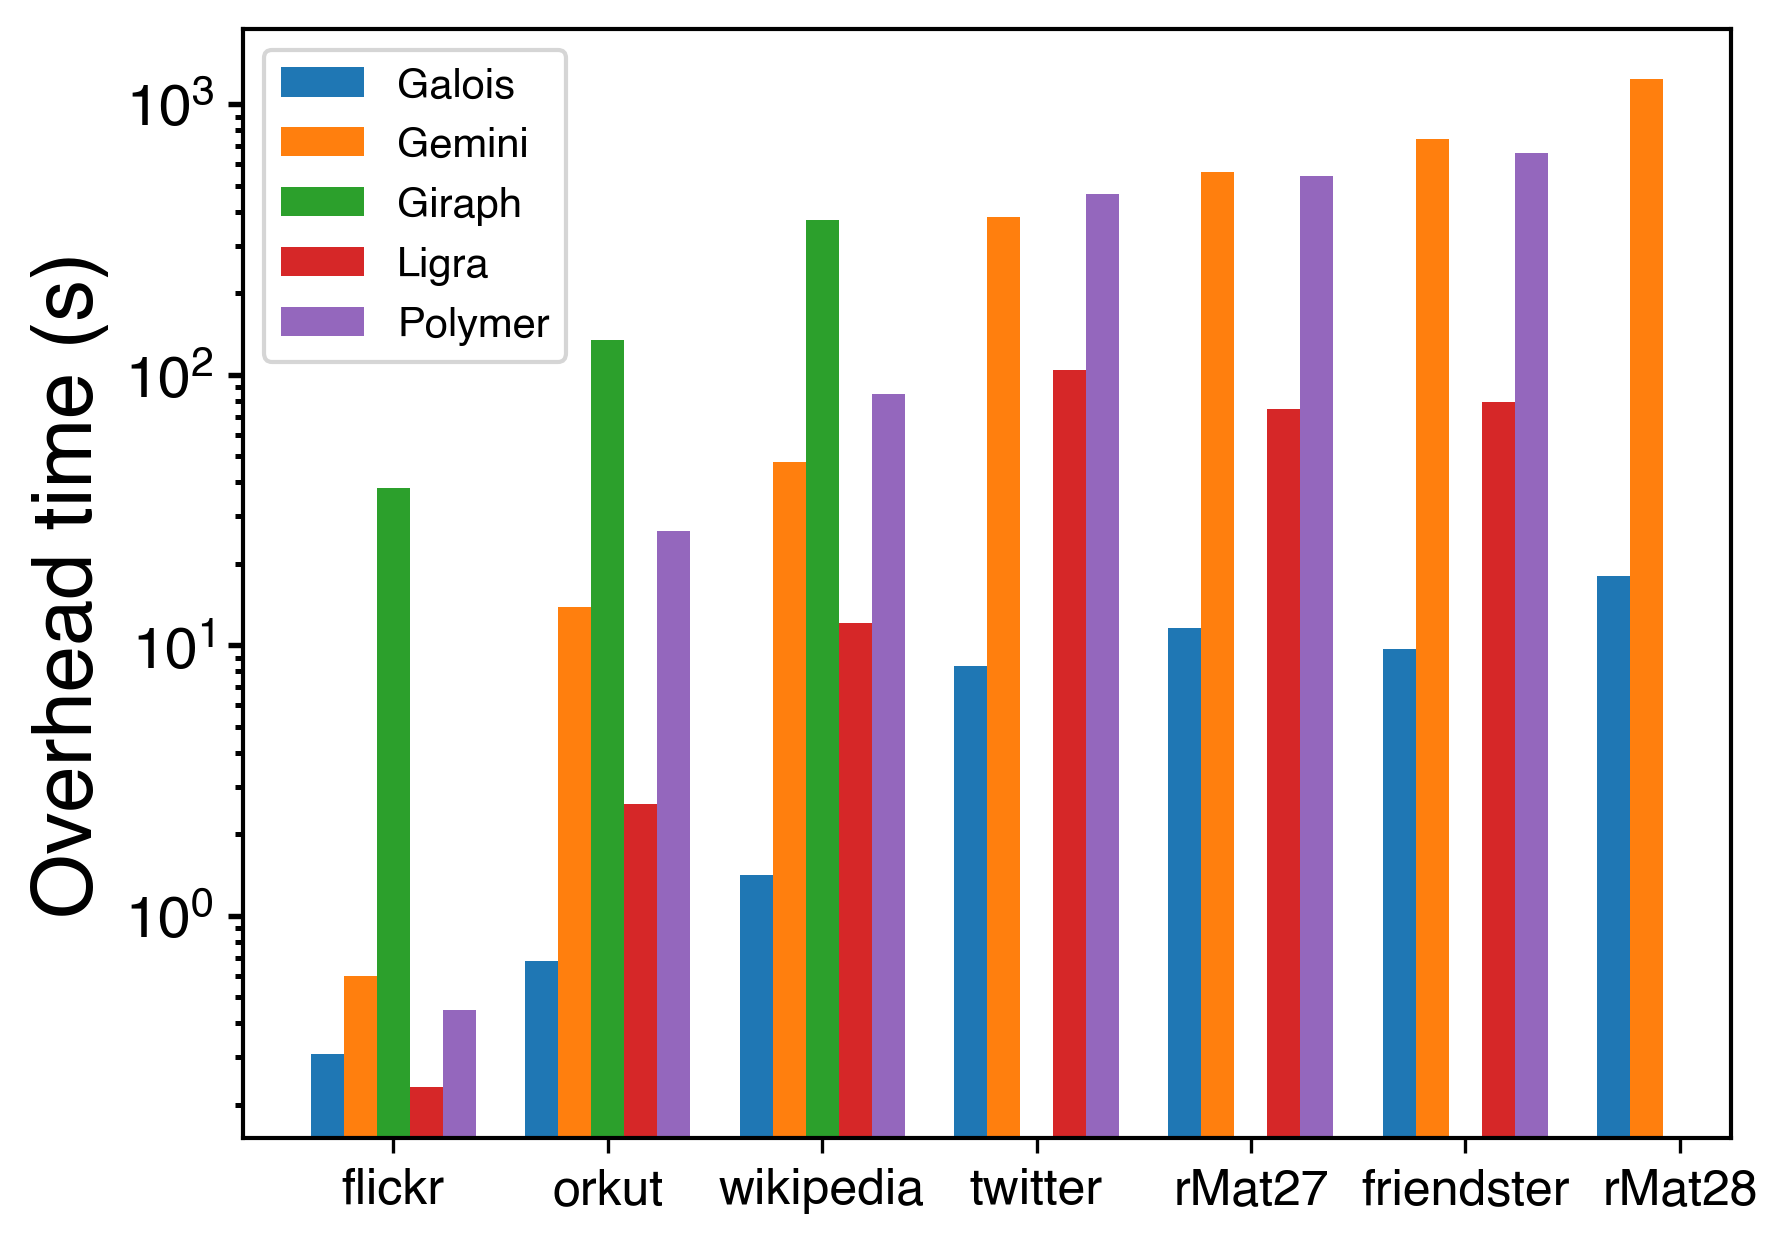
\includegraphics[width=\columnwidth]{../../plots/singleNodeSSSP_overheadTime.png}
	\caption{Overhead SSSP single node}
	\label{fig:singleNodeSSSP_overhead}
\end{figure}

\begin{figure}
	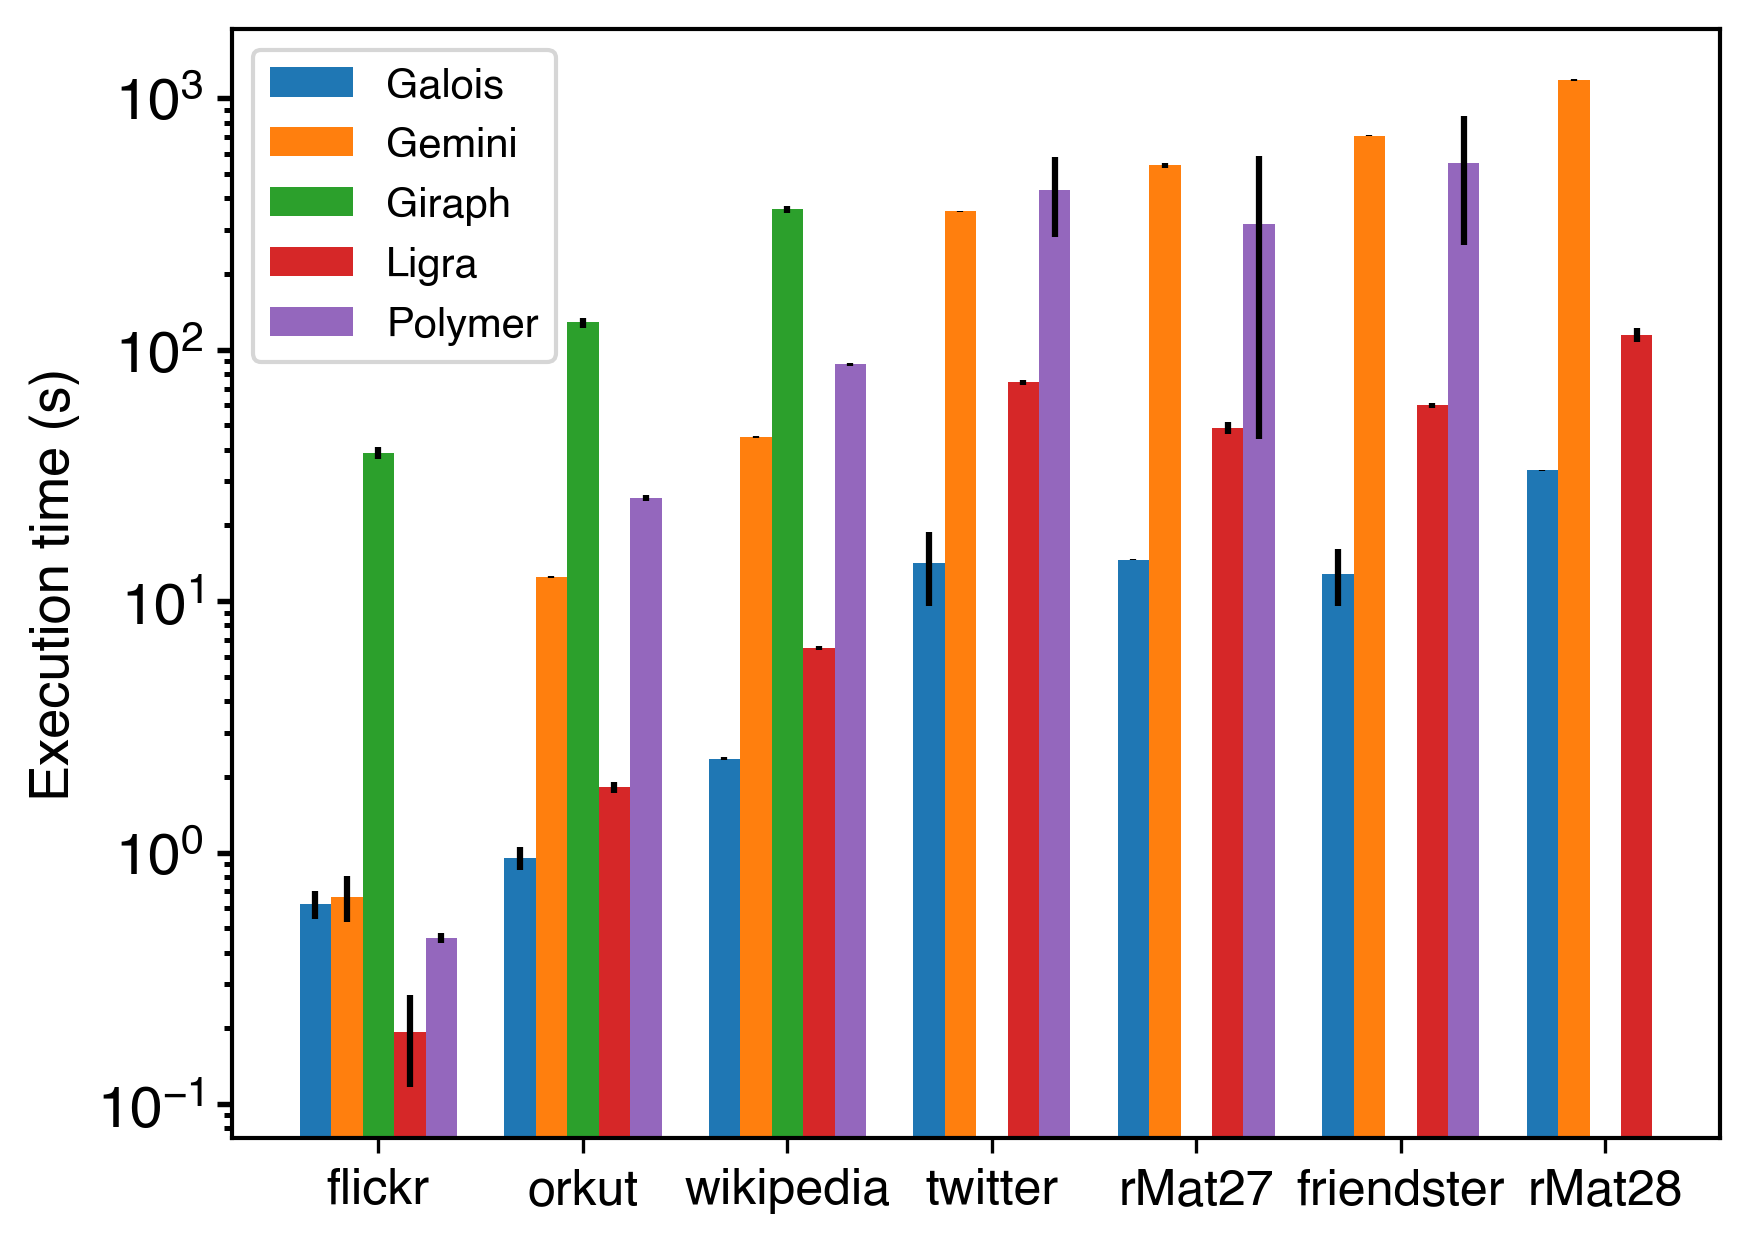
\includegraphics[width=\columnwidth]{../../plots/singleNodeBFS_execTime.png}
	\caption{Execution times for BFS on a single node}
	\label{fig:singleNodeBFS_exec}
\end{figure}

\begin{figure}
	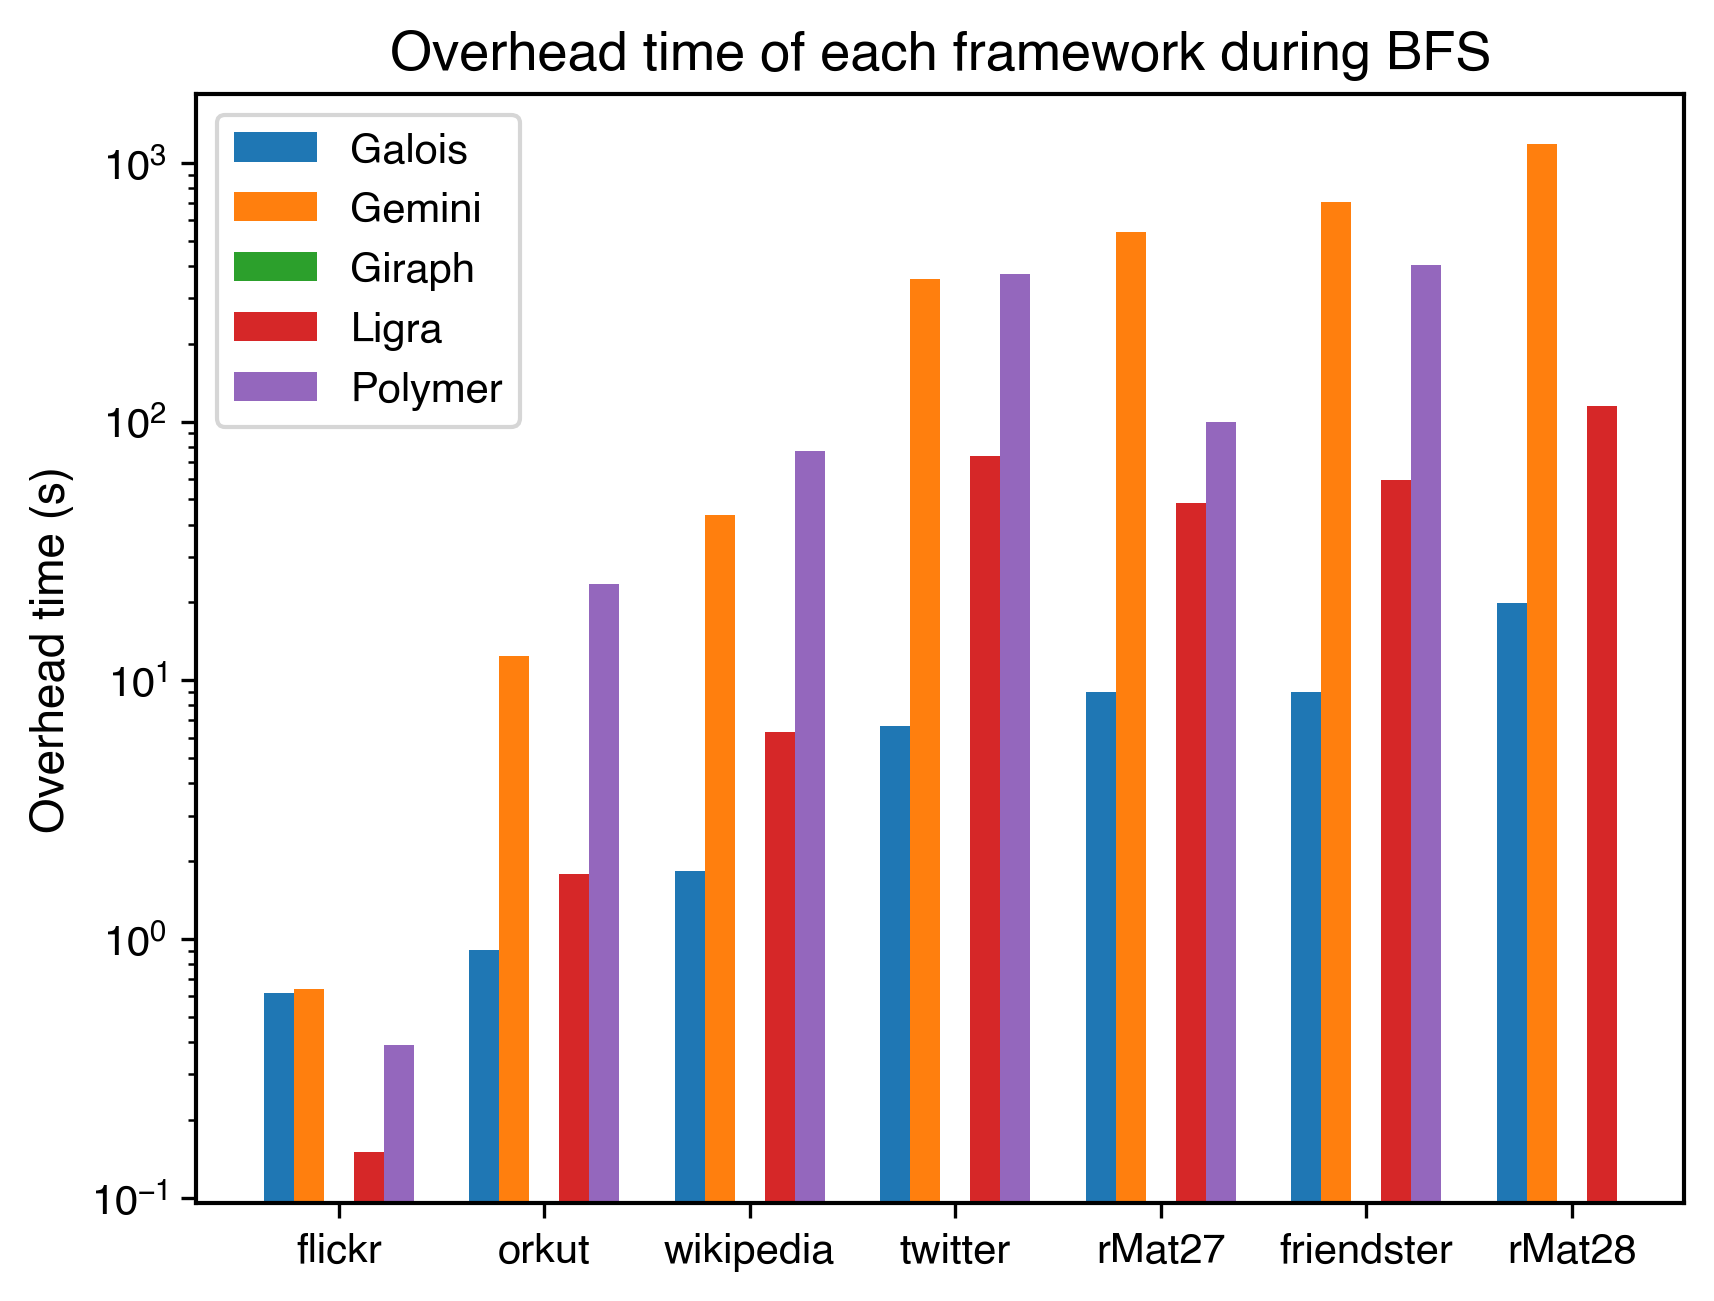
\includegraphics[width=\columnwidth]{../../plots/singleNodeBFS_overheadTime.png}
	\caption{Overhead BFS single node}
	\label{fig:singleNodeBFS_overhead}
\end{figure}

\begin{figure}
	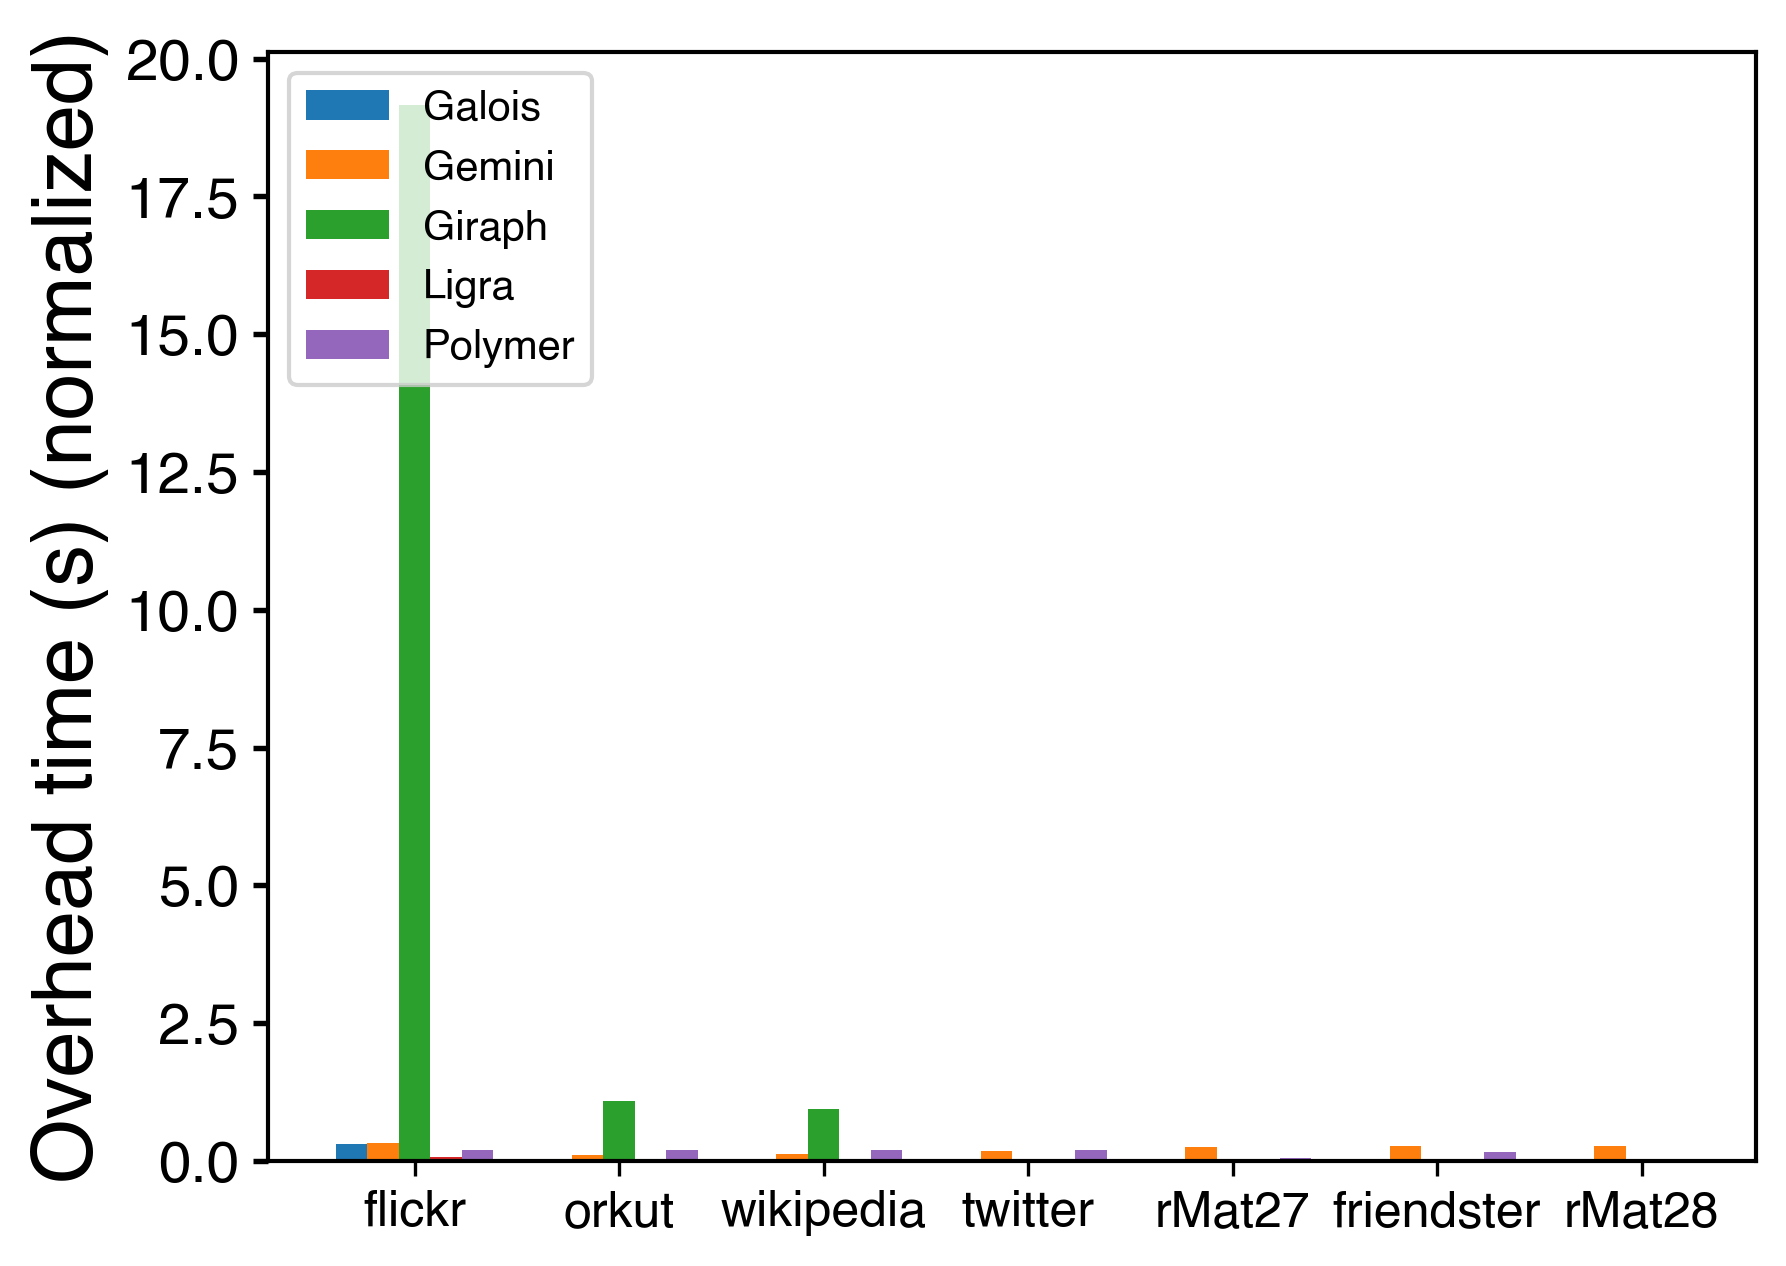
\includegraphics[width=\columnwidth]{../../plots/singleNodeBFS_overheadTimeNormalized.png}
	\caption{Normalized Overhead BFS single node}
	\label{fig:singleNodeBFS_overheadNormalized}
\end{figure}

hier erhoffe ich mir einen Vergleich der Ladezeiten und erwarte, dass Systeme wie Giraph, die erstmal auf irgendwas warten schlecht abschneiden.
Aber vielleicht ist auch die setup time bei gleichen frameworks zwischen verteilt und shared memory ganz interessant zu vergleichen. 
